\chapter{Resultados e Discussão}\label{sec:resultados}

\begin{dica}[Dica de metodologia científica: resultados e discussão]
Apresente primeiro os resultados, de forma objetiva e na ordem dos objetivos
específicos; depois discuta-os. Na discussão: interprete os números (o que significam?),
compare com os trabalhos do Referencial Teórico (confirmam ou contradizem?), relacione
com os objetivos e reconheça as limitações. Use tabelas, quadros e gráficos para os
dados e comente-os no texto \emph{sem repeti-los}: destaque o que importa. Toda
ilustração deve ser citada e explicada no texto. Resultados negativos ou inesperados
também são resultados e devem ser relatados e discutidos.
\end{dica}

\section{Tabelas}

Tabelas apresentam dados em que o \emph{número} é a informação central e seguem as
normas de apresentação tabular do \ac{ibge}. A \autoref{tab:exemplo} mostra o formato:
título acima, sem linhas verticais, fonte abaixo.

Nela, as colunas numéricas (tipo \texttt{S} do pacote \texttt{siunitx})
são alinhadas \emph{pela vírgula decimal}, mesmo quando os números têm quantidades
diferentes de dígitos e de casas decimais (``1234,5'' e ``62,8''; ``112,40'' e ``18,70''),
e os milhares são separados por ponto (``14.820''). A tabela ocupa toda a largura do
texto, e o título e o rodapé acompanham essa largura.

\begin{table}[htbp]
\begin{tabela}[\linewidth]{\caption{Desempenho das operações do sistema em cinco métricas}\label{tab:exemplo}}{\elaboracaopropria\nota{Média de 30 execuções. A coluna ``Variação'' compara com a versão anterior; valores negativos indicam melhoria.}}
  \begin{tabular*}{\linewidth}{@{\extracolsep{\fill}} l S[table-format=4.1] S[table-format=3.1] S[table-format=3.2] S[table-format=5.0] S[table-format=-2.1]}
    \toprule
    \textbf{Operação} & {\textbf{Tempo (ms)}} & {\textbf{Desvio (ms)}} & {\textbf{Memória (MB)}} & {\textbf{Vazão (req/s)}} & {\textbf{Variação (\%)}} \\
    \midrule
    Cadastro de usuário  &  184,3 &  12,6 &  41,25 &   520 &  -8,4 \\
    Autenticação         &   62,8 &   4,1 &  18,70 & 14820 & -12,0 \\
    Busca simples        &   95,5 &   7,9 &  33,05 &  9600 &  -3,2 \\
    Busca avançada       & 1234,5 &  85,2 & 112,40 &    78 &   5,7 \\
    Relatório mensal     & 2310,0 & 140,8 & 256,10 &    12 &  -0,6 \\
    Envio de arquivo     &  845,7 &  63,4 &  96,35 &   140 &   2,3 \\
    Exportação em CSV    &  530,2 &  38,9 &  64,80 &   260 & -21,5 \\
    Notificação por e-mail & 71,6 &   5,3 &  22,15 &  7800 &   0,0 \\
    Consulta de histórico &  318,9 & 24,7 &  52,45 &   460 &   9,8 \\
    \bottomrule
  \end{tabular*}
\end{tabela}
\end{table}

\begin{dica}[Dica de uso da classe: tabelas e quadros]
Se o conteúdo é \emph{numérico}, é \textbf{tabela}; se é \emph{textual}
(comparações, requisitos, definições, códigos), é \textbf{quadro}. As duas coisas têm
listas, numerações e formatos diferentes, por isso não classifique tudo como tabela. O
Apêndice~\ref{ap:tabelas} traz exemplos completos de tabelas e quadros bem formatados
e os principais ajustes (largura, alinhamento, notas, tabelas longas, células mescladas).
\end{dica}

\section{Gráficos}

Gráficos têm lista própria (``Lista de gráficos''). O \autoref{gra:exemplo} foi
desenhado no próprio \LaTeX\ com o pacote \texttt{pgfplots}, que funciona sobre o TikZ
(por isso o ambiente \texttt{axis} fica dentro de um \texttt{tikzpicture}), o que mantém
fontes e tamanhos coerentes com o texto.

\begin{grafico}[htbp]
  \begin{ilustracao}{\caption{Tempo médio de resposta por implementação}\label{gra:exemplo}}{\elaboracaopropria\nota{Média de 30 execuções.}}
    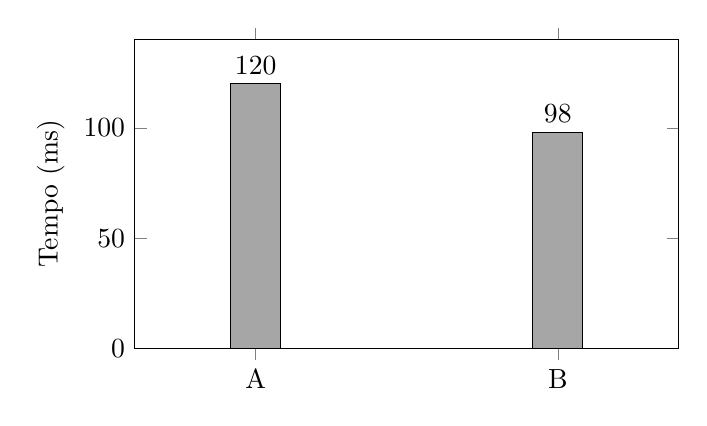
\begin{tikzpicture}
      \begin{axis}[ybar, width=0.7\linewidth, height=5.5cm, bar width=18pt,
          symbolic x coords={A, B}, xtick=data, ymin=0, ymax=140,
          ylabel={Tempo (ms)}, nodes near coords, enlarge x limits=0.4]
        \addplot[fill=black!35] coordinates {(A,120) (B,98)};
      \end{axis}
    \end{tikzpicture}
  \end{ilustracao}
\end{grafico}
